\documentclass{article}

\usepackage[paperwidth=8.5in,paperheight=11in,left=1.4in,
right=1in,top=1.3in, bottom=1.4in]{geometry}
\usepackage{sectsty, tikz, color, pgfplots}
\usetikzlibrary{shapes,arrows}
\usetikzlibrary{fit}
\begin{document}


\begin{figure}
  \centering
    \noindent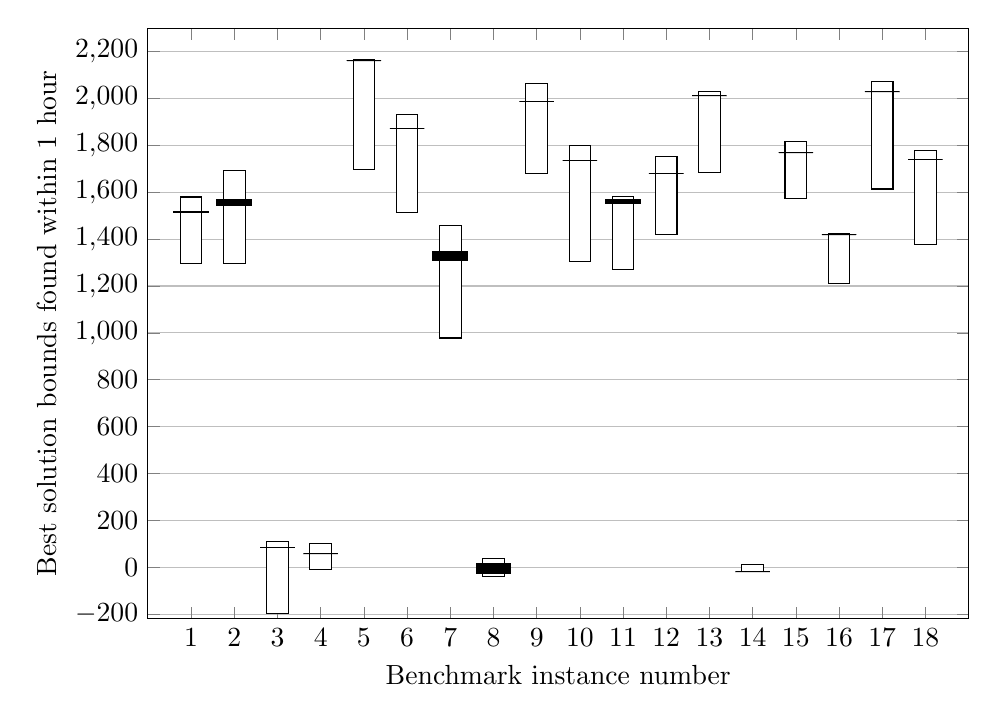
\begin{tikzpicture}

  \begin{axis}[width=0.99\textwidth, 
  height=0.749\textwidth,legend pos=north west, xmin=0, xmax=19, ymin=-220,
  ymax=2300.0, 
  only marks,
  xtick={1,2,3,4,5,6,7,8,9,10,11,12,13,14,15,16,17,18},
  ytick={-200, 0, 200, 400, 600, 800, 1000, 1200, 1400, 1600, 1800, 2000, 2200},
  ymajorgrids,
  log ticks with fixed point, 
    every axis legend/.append style={xshift=8pt, yshift=-5pt},
    ylabel=Best solution bounds found within 1 hour, xlabel=Benchmark instance number]

\draw[fill=white] (axis cs: 0.75,1297) rectangle (axis cs: 1.25, 1580);
\draw[fill=white] (axis cs: 1.75,1295) rectangle (axis cs: 2.25, 1694);
\draw[fill=white] (axis cs: 2.75,-197) rectangle (axis cs: 3.25, 108);
\draw[fill=white] (axis cs: 3.75,-11) rectangle (axis cs: 4.25, 100);
\draw[fill=white] (axis cs: 4.75,1699) rectangle (axis cs: 5.25, 2167);
\draw[fill=white] (axis cs: 5.75,1513) rectangle (axis cs: 6.25, 1930);
\draw[fill=white] (axis cs: 6.75,978) rectangle (axis cs: 7.25, 1459);
\draw[fill=white] (axis cs: 7.75,-41) rectangle (axis cs: 8.25, 36);
\draw[fill=white] (axis cs: 8.75,1679) rectangle (axis cs: 9.25, 2064);
\draw[fill=white] (axis cs: 9.75,1304) rectangle (axis cs: 10.25, 1799);
\draw[fill=white] (axis cs: 10.75,1270) rectangle (axis cs: 11.25, 1582);
\draw[fill=white] (axis cs: 11.75,1420) rectangle (axis cs: 12.25, 1752);
\draw[fill=white] (axis cs: 12.75,1683) rectangle (axis cs: 13.25, 2029);
\draw[fill=white] (axis cs: 13.75,-19) rectangle (axis cs: 14.25, 13);
\draw[fill=white] (axis cs: 14.75,1574) rectangle (axis cs: 15.25, 1815);
\draw[fill=white] (axis cs: 15.75,1212) rectangle (axis cs: 16.25, 1423);
\draw[fill=white] (axis cs: 16.75,1614) rectangle (axis cs: 17.25, 2074);
\draw[fill=white] (axis cs: 17.75,1377) rectangle (axis cs: 18.25, 1779);

\draw[fill=black] (axis cs: 0.6,1514) rectangle (axis cs: 1.4, 1516);
\draw[fill=black] (axis cs: 1.6,1544) rectangle (axis cs: 2.4, 1567);
\draw[fill=black] (axis cs: 2.6,86) rectangle (axis cs: 3.4, 86);
\draw[fill=black] (axis cs: 3.6,58) rectangle (axis cs: 4.4, 58);
\draw[fill=black] (axis cs: 4.6,2162) rectangle (axis cs: 5.4, 2162);
\draw[fill=black] (axis cs: 5.6,1874) rectangle (axis cs: 6.4, 1874);
\draw[fill=black] (axis cs: 6.6,1308) rectangle (axis cs: 7.4, 1348);
\draw[fill=black] (axis cs: 7.6,-26) rectangle (axis cs: 8.4, 16);
\draw[fill=black] (axis cs: 8.6,1989) rectangle (axis cs: 9.4, 1989);
\draw[fill=black] (axis cs: 9.6,1736) rectangle (axis cs: 10.4, 1736);
\draw[fill=black] (axis cs: 10.6,1551) rectangle (axis cs: 11.4, 1569);
\draw[fill=black] (axis cs: 11.6,1681) rectangle (axis cs: 12.4, 1681);
\draw[fill=black] (axis cs: 12.6,2012) rectangle (axis cs: 13.4, 2012);
\draw[fill=black] (axis cs: 13.6,-19) rectangle (axis cs: 14.4, -19);
\draw[fill=black] (axis cs: 14.6,1768) rectangle (axis cs: 15.4, 1768);
\draw[fill=black] (axis cs: 15.6,1418) rectangle (axis cs: 16.4, 1418);
\draw[fill=black] (axis cs: 16.6,2029) rectangle (axis cs: 17.4, 2029);
\draw[fill=black] (axis cs: 17.6,1740) rectangle (axis cs: 18.4, 1740);


  \end{axis}
\end{tikzpicture}
   \vspace{0.73em}
\end{figure}
\end{document}
